\documentclass[tikz]{standalone}
\usepackage{amsmath,amsfonts,amssymb,mathrsfs,tikz,fancyhdr}
\usepackage{fontspec}
\usepackage{unicode-math}
\usepackage{tikz}
\usepackage{tkz-euclide}
\usepackage{bidi}

\begin{document}

%% A ا B ٮ C ج D د E ه F ز G ح H ط J ك K ل L م M ن
\providecommand{\A} {ا}
\providecommand{\Ba}   {ٮ}
\providecommand{\Jīm}  {ج‍} % ZWJ U+200D
\providecommand{\Dal}  {د}
\providecommand{\Ha}   {ه‍} % ZWJ U+200D
\providecommand{\Z}    {ز}
\providecommand{\HH}   {ح}
\providecommand{\TT}   {ط}
\providecommand{\K}    {\tiny ڪ} %% Swash kaf U+06AA
\providecommand{\Lam}  {ل}
\providecommand{\M}    {م}
\providecommand{\N}    {ن}

\providecommand{\diam}{6pt}

\setmainfont[Script=Arabic,Mapping=arabicdigits]{Amiri}
\setmathfont{XITS Math}
% \newfontfamily\tikzfont{Amiri}
% \tikzset{every picture/.style={/utils/exec={\tikzfont}}}
% \tikzset{label style/.style={font=\tikzfont}}

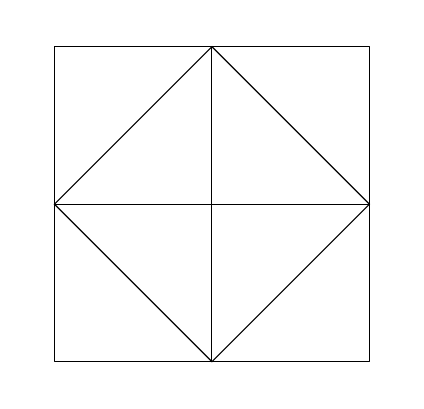
\begin{tikzpicture}[scale=2.0]
  % every node/.style={font=\fontspec{XITS Math}}]
  \tkzDefPoints{1/1/A, 0/1/TT, -1/1/B}
  \tkzDefPoints{-1/0/Z, 0/0/O, 1/0/H}
  \tkzDefPoints{-1/-1/D, 0/-1/HH, 1/-1/J}

  \node [above right] at (A)  {\RL{ا}};
  \node [above]       at (TT) {\RL{ط}};
  \node [above left]  at (B) {\RL{ب}};

  \node [left]       at (Z) {\RL{ز}};
  \node [above left] at (O) {\RL{ك‍}};  % ZWJ U+200D
  \node [right]      at (H) {\RL{ه‍}};  % ZWJ U+200D

  \node [below left]  at (D) {\RL{د}};
  \node [below]       at (HH){\RL{ح}};
  \node [below right] at (J){\RL{ج‍}};  % ZWJ U+200D

  \draw (TT) -- (Z) -- (HH) -- (H) -- cycle;
  \draw (TT) -- (HH);
  \draw (Z)  -- (H);

  % \tkzDefPoint(0,0){A}
  % \tkzDefPoint(2,0){B}
  % \tkzDefSquare(A,B)
  % \tkzGetPoints{C}{D}
  \tkzDrawPolygon(D,J,A,B)
  % \tkzDrawPoints(A,B,C,D)
  % \tkzLabelPoints[font=\fontspec{XITS Math}](ه,ا,ب,ز)
\end{tikzpicture}

\end{document}